% ============================================================================
%  Pr\'{e}sentation - Apprentissage F\'{e}d\'{e}r\'{e} pour la Pr\'{e}diction
%  de Maladies Cardiaques
%  Module : Optimisation | 2025--2026
%  Auteurs : Sifeddine LEGNIOUI & Youssef SARRAF
% ============================================================================
\documentclass[aspectratio=169,11pt]{beamer}

% ----- Packages -----
\usepackage[T1]{fontenc}
\usepackage[utf8]{inputenc}
\usepackage{lmodern} % Police propre
\usepackage{amsmath,amssymb}
\usepackage{booktabs}
\usepackage{graphicx}
\usepackage{tikz}
\usetikzlibrary{positioning, arrows.meta, shapes.geometric, calc, shadows}
\usepackage{xcolor}
\usepackage{pifont}

% ============================================================================
%  DESIGN MODERNE & CR\'{E}ATIF (DARK THEME TECH / AI)
% ============================================================================

% Couleurs
\definecolor{bgDark}{HTML}{1A1B26}        % Fond sombre tr\`{e}s moderne
\definecolor{panelBg}{HTML}{24283B}       % Fond des panneaux
\definecolor{fgWhite}{HTML}{A9B1D6}       % Texte normal (gris-bleu clair)
\definecolor{titleWhite}{HTML}{FFFFFF}    % Titres (blanc pur)
\definecolor{cyanAccent}{HTML}{7DCFFF}    % Accent primaire (Cyan)
\definecolor{magentaAccent}{HTML}{F7768E} % Accent secondaire (Magenta)
\definecolor{greenAccent}{HTML}{9ECE6A}   % Accent tertiaire (Vert)

\setbeamercolor{background canvas}{bg=bgDark}
\setbeamercolor{normal text}{fg=fgWhite}
\setbeamercolor{structure}{fg=cyanAccent}
\setbeamercolor{itemize item}{fg=cyanAccent}
\setbeamercolor{itemize subitem}{fg=magentaAccent}

% Titres des slides (Frametitle Custom)
\setbeamertemplate{frametitle}{
    \vspace{0.2cm}
    \begin{tikzpicture}[remember picture, overlay]
        \fill[panelBg] (current page.north west) rectangle ([yshift=-1.2cm]current page.north east);
        \draw[cyanAccent, thick] (current page.north west) ++(0, -1.2cm) -- ++(\paperwidth, 0);
        \node[anchor=west, font=\Large\bfseries, text=titleWhite] at ([xshift=0.5cm, yshift=-0.6cm]current page.north west) {\insertframetitle};
        \node[anchor=east, font=\footnotesize\bfseries, text=magentaAccent] at ([xshift=-0.5cm, yshift=-0.6cm]current page.north east) {PROJET FL};
    \end{tikzpicture}
    \vspace{0.6cm}
}

% Footer Custom
\setbeamertemplate{footline}{
    \begin{tikzpicture}[remember picture, overlay]
        \draw[panelBg, thick] (current page.south west) ++(0, 0.6cm) -- ++(\paperwidth, 0);
        \node[anchor=west, font=\footnotesize, text=fgWhite] at ([xshift=0.5cm, yshift=0.3cm]current page.south west) {Sifeddine \textsc{Legnioui} \& Youssef \textsc{Sarraf} \quad $\vert$ \quad Optimisation};
        \node[anchor=east, font=\footnotesize\bfseries, text=cyanAccent] at ([xshift=-0.5cm, yshift=0.3cm]current page.south east) {\insertframenumber~-~\inserttotalframenumber};
    \end{tikzpicture}
}
\setbeamertemplate{navigation symbols}{}

% Blocs Custom
\setbeamercolor{block title}{bg=panelBg, fg=cyanAccent}
\setbeamercolor{block body}{bg=panelBg!50!bgDark, fg=fgWhite}
\setbeamercolor{block title alerted}{bg=panelBg, fg=magentaAccent}
\setbeamercolor{block body alerted}{bg=panelBg!50!bgDark, fg=fgWhite}
\setbeamercolor{block title example}{bg=panelBg, fg=greenAccent}
\setbeamercolor{block body example}{bg=panelBg!50!bgDark, fg=fgWhite}
\setbeamertemplate{blocks}[rounded][shadow=true]

% ============================================================================
%  D\'{E}BUT DU DOCUMENT
% ============================================================================

\begin{document}

% ----------------------------------------------------------------------------
% 1. PAGE DE TITRE CR\'{E}ATIVE
% ----------------------------------------------------------------------------
\begin{frame}[plain]
\begin{tikzpicture}[remember picture, overlay]
    % Particules / Nodes en arri\`{e}re-plan
    \foreach \i in {1,...,15} {
        \node[circle, fill=cyanAccent, opacity=0.15, inner sep=2pt] (n\i) at (rand*7+7, rand*4-2) {};
    }
    \foreach \i in {1,...,14} {
        \draw[cyanAccent, opacity=0.08, thick] (n\i) -- (n\the\numexpr\i+1\relax);
    }
    % Cercle design
    \draw[magentaAccent, opacity=0.2, line width=1mm] (current page.south west) ++(2,1) circle (3cm);
    \draw[cyanAccent, opacity=0.1, line width=2mm] (current page.north east) ++(-1,-1) circle (4cm);

    % Titre central
    \node[anchor=center, align=center] at (current page.center) {
        \color{cyanAccent}\rule{8cm}{1.5pt} \\[0.4cm]
        \color{titleWhite}\Huge\bfseries APPRENTISSAGE F\'{E}D\'{E}R\'{E} \\[0.3cm]
        \color{fgWhite}\Large Pr\'{e}diction de Maladies Cardiaques \\[0.4cm]
        \color{cyanAccent}\rule{8cm}{1.5pt} \\[0.8cm]
        \color{titleWhite}\large Sifeddine \textsc{Legnioui} \& Youssef \textsc{Sarraf} \\[0.2cm]
        \color{magentaAccent}\normalsize Module : Optimisation -- 2025/2026
    };
\end{tikzpicture}
\end{frame}

% ----------------------------------------------------------------------------
% 2. PLAN
% ----------------------------------------------------------------------------
\begin{frame}{Plan de la pr\'{e}sentation}
  \tableofcontents[hideallsubsections]
\end{frame}

% ============================================================================
\section{1. Contexte \& Probl\'{e}matique}
% ============================================================================

\begin{frame}{Le Contexte : La Sant\'{e} \& L'IA}
  \begin{columns}
    \begin{column}{0.5\textwidth}
      \begin{block}{Une opportunit\'{e} massive}
        L'intelligence artificielle peut r\'{e}volutionner le diagnostic m\'{e}dical (d\'{e}tection pr\'{e}coce, m\'{e}decine personnalis\'{e}e).
      \end{block}
      \begin{alertblock}{La R\'{e}alit\'{e} du Terrain}
        \begin{itemize}
          \item Les donn\'{e}es sont bloqu\'{e}es dans les h\^{o}pitaux.
          \item M\'{e}fiance quant au partage de donn\'{e}es sensibles.
          \item Des lois strictes s'appliquent (RGPD, HIPAA).
        \end{itemize}
      \end{alertblock}
    \end{column}
    \begin{column}{0.45\textwidth}
      \begin{center}
        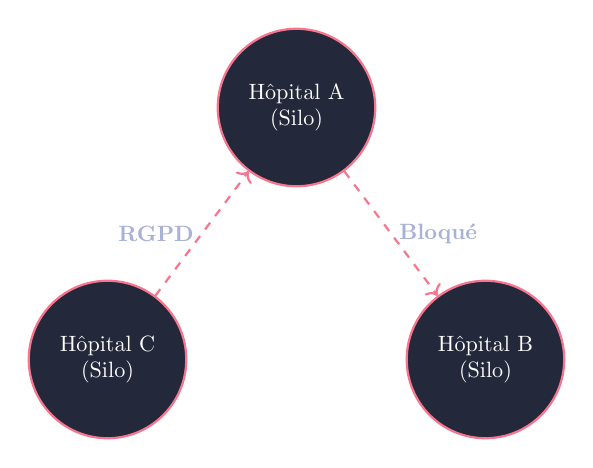
\begin{tikzpicture}[scale=0.8, transform shape]
            \node[circle, draw=magentaAccent, fill=panelBg, thick, minimum size=2.5cm, align=center, text=titleWhite] (A) at (0,3) {H\^{o}pital A\\(Silo)};
            \node[circle, draw=magentaAccent, fill=panelBg, thick, minimum size=2.5cm, align=center, text=titleWhite] (B) at (3,-1) {H\^{o}pital B\\(Silo)};
            \node[circle, draw=magentaAccent, fill=panelBg, thick, minimum size=2.5cm, align=center, text=titleWhite] (C) at (-3,-1) {H\^{o}pital C\\(Silo)};
            \draw[magentaAccent, thick, dashed, ->] (A) -- (B) node[midway, right, text=fgWhite] {\textbf{Bloqu\'{e}}};
            \draw[magentaAccent, thick, dashed, ->] (C) -- (A) node[midway, left, text=fgWhite] {\textbf{RGPD}};
        \end{tikzpicture}
      \end{center}
    \end{column}
  \end{columns}
\end{frame}

\begin{frame}{La Solution : L'Apprentissage F\'{e}d\'{e}r\'{e} (FL)}
  \begin{exampleblock}{Le Changement de Paradigme}
    \textit{"Ne d\'{e}placez pas les donn\'{e}es vers le mod\`{e}le. D\'{e}placez le mod\`{e}le vers les donn\'{e}es."}
  \end{exampleblock}
  \vspace{0.4cm}
  
  \begin{itemize}
    \item \textbf{Collaboration s\'{e}curis\'{e}e :} Plusieurs h\^{o}pitaux entra\^{i}nent une IA ensemble.
    \item \textbf{Z\'{e}ro fuite :} Aucune donn\'{e}e patient n'est jamais transmise sur le r\'{e}seau.
    \item \textbf{Poids uniquement :} Seuls les \emph{param\`{e}tres math\'{e}matiques} du r\'{e}seau de neurones sont partag\'{e}s et fusionn\'{e}s.
  \end{itemize}
\end{frame}

\begin{frame}{Le Cahier des Charges (Option 4)}
  Notre projet s'inscrit rigoureusement dans les exigences du Professeur :
  \vspace{0.3cm}
  \begin{columns}
    \begin{column}{0.48\textwidth}
      \begin{itemize}
          \item[\color{cyanAccent}\ding{51}] Donn\'{e}es tabulaires (Maladies cardiaques)
          \item[\color{cyanAccent}\ding{51}] R\'{e}seau : Perceptron Multicouche (MLP)
          \item[\color{cyanAccent}\ding{51}] 8 clients simul\'{e}s (H\^{o}pitaux)
      \end{itemize}
    \end{column}
    \begin{column}{0.48\textwidth}
      \begin{itemize}
          \item[\color{cyanAccent}\ding{51}] 4 Algorithmes f\'{e}d\'{e}r\'{e}s test\'{e}s
          \item[\color{cyanAccent}\ding{51}] Partitions IID vs Non-IID
          \item[\color{cyanAccent}\ding{51}] M\'{e}triques claires (Accuracy, Perte)
      \end{itemize}
    \end{column}
  \end{columns}
\end{frame}

% ============================================================================
\section{2. M\'{e}thodologie \& Architecture}
% ============================================================================

\begin{frame}{L'Architecture F\'{e}d\'{e}r\'{e}e : Topologie \'{E}toile}
  \begin{figure}
    \centering
    \resizebox{0.7\textwidth}{!}{%
    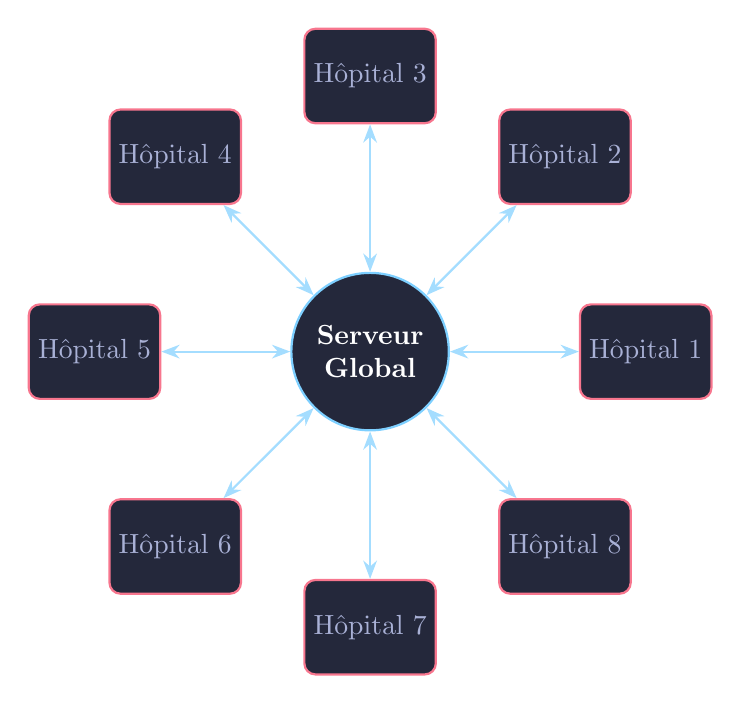
\begin{tikzpicture}[
        server/.style={circle, draw=cyanAccent, fill=panelBg, thick, minimum size=2cm, align=center, font=\bfseries, text=titleWhite},
        client/.style={rectangle, rounded corners, draw=magentaAccent, fill=panelBg, thick, minimum size=1.2cm, align=center, text=fgWhite},
        arrow/.style={<->, >=Stealth, thick, cyanAccent!70}
      ]
      \node[server] (S) {Serveur\\Global};
      \foreach \a/\i in {0/1, 45/2, 90/3, 135/4, 180/5, 225/6, 270/7, 315/8} {
         \node[client] (H\i) at (\a:3.5cm) {H\^{o}pital \i};
         \draw[arrow] (S) -- (H\i);
      }
    \end{tikzpicture}
    }
  \end{figure}
\end{frame}

\begin{frame}{Le Dataset : Heart Disease UCI}
  \begin{block}{Description du jeu de donn\'{e}es}
    \begin{itemize}
      \item \textbf{Taille :} 1\,025 patients.
      \item \textbf{13 Attributs cliniques :} \^{A}ge, sexe, type de douleur (CP), cholest\'{e}rol, ECG, etc.
      \item \textbf{Cible :} Classification binaire (0 = Sain, 1 = Maladie Cardiaque).
    \end{itemize}
  \end{block}
  \vspace{0.2cm}
  
  \textbf{Pr\'{e}traitement r\'{e}alis\'{e} :}
  \begin{itemize}
    \item \textbf{Encodage One-Hot} sur les variables cat\'{e}gorielles.
    \item \textbf{Standardisation Z-score} sur les variables continues pour faciliter l'entra\^{i}nement.
    \item \emph{R\'{e}sultat :} Un vecteur de taille 23 pour chaque patient.
  \end{itemize}
\end{frame}

\begin{frame}{L'Architecture du Mod\`{e}le (MLP)}
  Un Perceptron Multicouche l\'{e}ger et optimal pour ce jeu de donn\'{e}es.
  \vspace{0.3cm}
  
  \begin{center}
    
\begin{tikzpicture}[scale=0.9, transform shape,
      node/.style={circle, draw=cyanAccent, fill=panelBg, minimum size=0.8cm, text=titleWhite},
      box/.style={rectangle, rounded corners, draw=magentaAccent, fill=panelBg, minimum width=2.5cm, minimum height=1cm, align=center, text=titleWhite}
    ]
      \node[box] (in) at (0,0) {Entr\'{e}e\\(23 Features)};
      \node[box] (h1) at (3.5,0) {Couche Cach\'{e}e 1\\(64 Neurones)};
      \node[box] (h2) at (7.5,0) {Couche Cach\'{e}e 2\\(32 Neurones)};
      \node[box] (out) at (11.5,0) {Sortie\\(1 Neurone)};
      
      \draw[->, cyanAccent, thick] (in) -- (h1);
      \draw[->, cyanAccent, thick] (h1) -- (h2);
      \draw[->, cyanAccent, thick] (h2) -- (out);
      
      \node[below=0.2cm of h1, text=fgWhite, font=\footnotesize] {ReLU + Dropout (0.2)};
      \node[below=0.2cm of h2, text=fgWhite, font=\footnotesize] {ReLU + Dropout (0.2)};
      \node[below=0.2cm of out, text=fgWhite, font=\footnotesize] {BCEWithLogitsLoss};
    \end{tikzpicture}
  \end{center}
  
  \vspace{0.4cm}
  \begin{itemize}
    \item \textbf{Taille Totale :} $\sim$2\,600 param\`{e}tres.
    \item \textbf{Poids m\'{e}moire :} Moins de 11 Ko (tr\`{e}s rapide \`{a} envoyer aux h\^{o}pitaux).
  \end{itemize}
\end{frame}

% ============================================================================
\section{3. Sc\'{e}narios de R\'{e}partition (IID vs Non-IID)}
% ============================================================================

\begin{frame}{R\'{e}partition IID : Le Monde Id\'{e}al}
  \begin{columns}
    \begin{column}{0.5\textwidth}
      \begin{block}{IID (Independent and Identically Distributed)}
        Chaque h\^{o}pital re\c{c}oit un \'{e}chantillon parfaitement repr\'{e}sentatif de la population globale (50\% malades, 50\% sains).
      \end{block}
      \begin{itemize}
        \item Simule des h\^{o}pitaux g\'{e}n\'{e}ralistes.
        \item Excellent pour la convergence algorithmique.
      \end{itemize}
    \end{column}
    \begin{column}{0.45\textwidth}
      \begin{figure}
        \centering
        % PLACEHOLDER POUR L'IMAGE DE DISTRIBUTION IID
        \includegraphics[width=0.9\textwidth]{example-image}
        \caption{\color{fgWhite}\footnotesize Distribution IID des classes}
      \end{figure}
    \end{column}
  \end{columns}
\end{frame}

\begin{frame}{R\'{e}partition Non-IID : Le Monde R\'{e}el}
  \begin{columns}
    \begin{column}{0.5\textwidth}
      \begin{alertblock}{Non-IID (Distribution de Dirichlet $\alpha=0.5$)}
        Certains h\^{o}pitaux n'ont presque que des patients malades (Sp\'{e}cialis\'{e}s), d'autres que des cas sains.
      \end{alertblock}
      \begin{itemize}
        \item C'est le d\'{e}fi principal du FL !
        \item Cr\'{e}e un "Client Drift" : chaque h\^{o}pital se sp\'{e}cialise trop sur ses propres patients.
      \end{itemize}
    \end{column}
    \begin{column}{0.45\textwidth}
      \begin{figure}
        \centering
        % PLACEHOLDER POUR L'IMAGE DE DISTRIBUTION NON-IID
        \includegraphics[width=0.9\textwidth]{example-image}
        \caption{\color{fgWhite}\footnotesize Distribution Non-IID asym\'{e}trique}
      \end{figure}
    \end{column}
  \end{columns}
\end{frame}

% ============================================================================
\section{4. Les Algorithmes de la F\'{e}d\'{e}ration}
% ============================================================================

\begin{frame}{4 Approches Algorithmiques}
  \begin{enumerate}
    \item \textbf{Local SGD (L'Isolation) :}
          Aucun serveur central. Chaque h\^{o}pital s'entra\^{i}ne dans son coin. R\'{e}f\'{e}rence basse (Baseline).
    \vspace{0.2cm}
    \item \textbf{FedAvg (Le Standard de Google) :}
          Le serveur collecte les mod\`{e}les locaux, en fait une simple moyenne, et redistribue la moyenne.
    \vspace{0.2cm}
    \item \textbf{FedAdam (L'Acc\'{e}l\'{e}ration Adaptative) :}
          Le serveur garde une m\'{e}moire (inertie) des agr\'{e}gations pr\'{e}c\'{e}dentes. Tr\`{e}s rapide quand les donn\'{e}es sont propres (IID).
    \vspace{0.2cm}
    \item \textbf{FedProx (Le Bouclier Non-IID) :}
          Ajoute un \emph{ressort math\'{e}matique} (R\'{e}gularisation Proximale) : emp\^{e}che un h\^{o}pital d'alt\'{e}rer le mod\`{e}le trop radicalement.
  \end{enumerate}
\end{frame}

% ============================================================================
\section{5. R\'{e}sultats \& Analyses}
% ============================================================================

\begin{frame}{R\'{e}sultats : Performance Globale (Accuracy)}
  \begin{table}
    \centering
    \color{fgWhite}
    \begin{tabular}{lcc}
      \toprule
      \textbf{\color{cyanAccent}Algorithme} & \textbf{\color{cyanAccent}Pr\'{e}cision IID} & \textbf{\color{cyanAccent}Pr\'{e}cision Non-IID} \\
      \midrule
      Local SGD  & 81.3\% & \textcolor{magentaAccent}{\textbf{62.1\%}} \\
      FedAvg     & 91.8\% & 91.3\% \\
      FedAdam    & \textcolor{greenAccent}{\textbf{92.4\%}} & 90.7\% \\
      FedProx    & 91.8\% & \textcolor{greenAccent}{\textbf{91.7\%}} \\
      \bottomrule
    \end{tabular}
  \end{table}
  
  \vspace{0.3cm}
  \begin{itemize}
    \item \textbf{La collaboration fonctionne :} Passer de 62\% \`{a} plus de 91\% en Non-IID sans bouger une seule donn\'{e}e patient.
    \item \textbf{Victoire de FedProx :} C'est le plus robuste face au d\'{e}s\'{e}quilibre massif des h\^{o}pitaux.
  \end{itemize}
\end{frame}

\begin{frame}{R\'{e}sultats : Courbes d'Apprentissage (Loss)}
  \begin{columns}
    \begin{column}{0.5\textwidth}
      \begin{figure}
        \centering
        % PLACEHOLDER POUR COURBES IID
        \includegraphics[width=\textwidth]{example-image}
        \caption{\color{fgWhite}\footnotesize Pertes (Loss) en IID}
      \end{figure}
    \end{column}
    \begin{column}{0.5\textwidth}
      \begin{figure}
        \centering
        % PLACEHOLDER POUR COURBES NON-IID
        \includegraphics[width=\textwidth]{example-image}
        \caption{\color{fgWhite}\footnotesize Pertes (Loss) en Non-IID}
      \end{figure}
    \end{column}
  \end{columns}
\end{frame}

\begin{frame}{Analyse de la Divergence Locale}
  \begin{columns}
    \begin{column}{0.5\textwidth}
      \begin{block}{Le Ph\'{e}nom\`{e}ne de "D\'{e}rive"}
        L'analyse de la norme $L_2$ prouve que FedProx maintient les mod\`{e}les hospitaliers "group\'{e}s", l\`{a} o\`{u} Local SGD explose.
      \end{block}
    \end{column}
    \begin{column}{0.45\textwidth}
      \begin{figure}
        \centering
        % PLACEHOLDER POUR COURBE DIVERGENCE
        \includegraphics[width=\textwidth]{example-image}
        \caption{\color{fgWhite}\footnotesize \'{E}volution de la Divergence $L_2$}
      \end{figure}
    \end{column}
  \end{columns}
\end{frame}

\begin{frame}{Efficacit\'{e} R\'{e}seau \& Co\^{u}t de Communication}
  \begin{exampleblock}{Un syst\`{e}me taill\'{e} pour le monde r\'{e}el}
    \begin{itemize}
        \item \textbf{1 \'{e}change H\^{o}pital-Serveur :} $\sim$10.6 Ko
        \item \textbf{Volume pour 1 Round (8 H\^{o}pitaux) :} $\sim$160 Ko
        \item \textbf{Volume Total (15 Rounds) :} \textbf{$\sim$2.45 Mo}
    \end{itemize}
  \end{exampleblock}
  \vspace{0.4cm}
  \textit{Conclusion :} Le poids total de tout l'entra\^{i}nement collaboratif sur Internet p\`{e}se \textbf{moins lourd qu'une seule photo sur smartphone}. C'est id\'{e}al pour les infrastructures IT des h\^{o}pitaux.
\end{frame}

% ============================================================================
\section{6. Conclusion \& Perspectives}
% ============================================================================

\begin{frame}{Conclusion G\'{e}n\'{e}rale}
  \begin{enumerate}
    \item \textbf{Mission Accomplie :} R\'{e}ussite du diagnostic f\'{e}d\'{e}r\'{e} (Heart Disease) en respectant \`{a} 100\% la vie priv\'{e}e.
    \item \textbf{Option 4 Valid\'{e}e :} Tabulaire, MLP, 8 clients, 4 algorithmes, IID \& Non-IID ont \'{e}t\'{e} analys\'{e}s.
    \item \textbf{Algorithme Gagnant :} \textbf{FedProx} d\'{e}montre une stabilit\'{e} sup\'{e}rieure en condition r\'{e}elle h\'{e}t\'{e}rog\`{e}ne.
  \end{enumerate}
  \vspace{0.4cm}
  \begin{block}{Perspectives Futures}
    \begin{itemize}
        \item Ajouter la \emph{Confidentialit\'{e} Diff\'{e}rentielle} (bruit statique) pour bloquer les attaques de r\'{e}tro-ing\'{e}nierie.
        \item Passer \`{a} l'imagerie m\'{e}dicale (CNN, IRM).
    \end{itemize}
  \end{block}
\end{frame}

\begin{frame}[plain]
  \begin{tikzpicture}[remember picture, overlay]
    \fill[bgDark] (current page.south west) rectangle (current page.north east);
    
    \draw[cyanAccent, opacity=0.3, line width=2mm] (current page.center) circle (3cm);
    \draw[magentaAccent, opacity=0.3, line width=1mm] (current page.center) circle (4cm);
    
    \node[anchor=center, align=center] at (current page.center) {
        \color{titleWhite}\Huge\bfseries MERCI DE VOTRE ATTENTION \\[0.8cm]
        \color{cyanAccent}\Large Avez-vous des questions ?
    };
  \end{tikzpicture}
\end{frame}

\end{document}
